\documentclass[10pt,oneside]{article}
\usepackage[T1]{fontenc}
\usepackage[utf8]{inputenc}
% \usepackage{lmodern}
%\usepackage[adobe-utopia,uppercase=upright,greeklowercase=upright]{mathdesign}
\usepackage[adobe-utopia]{mathdesign}
%\usepackage{minionpro}
% \usepackage{pifont}
% \usepackage{amssymb}
\usepackage{amsmath}
\usepackage[francais]{babel}
% \usepackage[francais]{varioref}
\usepackage[dvips]{graphicx}

\usepackage{framed}
\usepackage[normalem]{ulem}
\usepackage{fancyhdr}
\usepackage{titlesec}
\usepackage{vmargin}
\usepackage{longtable}

\usepackage{ifthen}


%\usepackage{epsfig}
\usepackage{subfig}

\usepackage{multirow}
\usepackage{multicol} % Portions de texte en colonnes
\usepackage{flafter}%floatants après la référence



\usepackage{color}
\usepackage{colortbl}


\definecolor{gris25}{gray}{0.75}
\definecolor{bleu}{RGB}{18,33,98}
\definecolor{bleuf}{RGB}{42,94,171}
\definecolor{bleuc}{RGB}{231,239,247}
\definecolor{rougef}{RGB}{185,18,27}
\definecolor{rougec}{RGB}{255,230,231}
\definecolor{vertf}{RGB}{103,126,82}
\definecolor{vertc}{RGB}{220,255,191}

\newenvironment{rem}[1][\hsize]%
{%
    \def\FrameCommand
    {%
\rotatebox{90}{\textit{\textsf{Remarque}}} 
        {\color{bleuf}\vrule width 3pt}%
        \hspace{0pt}%must no space.
        \fboxsep=\FrameSep\colorbox{bleuc}%
    }%
    \MakeFramed{\hsize#1\advance\hsize-\width\FrameRestore}%
}%
{\endMakeFramed}%


\newenvironment{savoir}[1][\hsize]%
{%
    \def\FrameCommand
    {%
\rotatebox{90}{\textit{\textsf{Savoir}}} 
        {\color{bleuf}\vrule width 3pt}%
        \hspace{0pt}%must no space.
        \fboxsep=\FrameSep\colorbox{bleuc}%
    }%
    \MakeFramed{\hsize#1\advance\hsize-\width\FrameRestore}%
}%
{\endMakeFramed}%

\newenvironment{prob}[1][\hsize]%
{%
    \def\FrameCommand%
    {%
\rotatebox{90}{\textit{\textsf{ Problématique}}} 
        {\color{rougef}\vrule width 3pt}%
        \hspace{0pt}%must no space.
        \fboxsep=\FrameSep\colorbox{rougec}%
    }%
    \MakeFramed{\hsize#1\advance\hsize-\width\FrameRestore}%
}%
{\endMakeFramed}%

\newenvironment{obj}[1][\hsize]%
{%
    \def\FrameCommand%
    {%
\rotatebox{90}{\textit{\textsf{ $\;$}}} 
        {\color{rougef}\vrule width 3pt}%
        \hspace{0pt}%must no space.
        \fboxsep=\FrameSep\colorbox{rougec}%
    }%
    \MakeFramed{\hsize#1\advance\hsize-\width\FrameRestore}%
}%
{\endMakeFramed}%

\newenvironment{defi}[1][\hsize]%
{%
    \def\FrameCommand%
    {%
\rotatebox{90}{\textit{\textsf{Définition\\}}} 
        {\color{bleuf}\vrule width 3pt}%
        \hspace{0pt}%must no space.
        \fboxsep=\FrameSep\colorbox{bleuc}%
    }%
    \MakeFramed{\hsize#1\advance\hsize-\width\FrameRestore}%
}%
{\endMakeFramed}%


\newenvironment{hypo}[1][\hsize]%
{%
    \def\FrameCommand%
    {%
\rotatebox{90}{\textit{\textsf{Hypothèse\\}}} 
        {\color{bleuf}\vrule width 3pt}%
        \hspace{0pt}%must no space.
        \fboxsep=\FrameSep\colorbox{bleuc}%
    }%
    \MakeFramed{\hsize#1\advance\hsize-\width\FrameRestore}%
}%
{\endMakeFramed}%


\newenvironment{prop}[1][\hsize]%
{%
    \def\FrameCommand%
    {%
\rotatebox{90}{\textit{\textsf{Propriété\\}}} 
        {\color{bleuf}\vrule width 3pt}%
        \hspace{0pt}%must no space.
        \fboxsep=\FrameSep\colorbox{bleuc}%
    }%
    \MakeFramed{\hsize#1\advance\hsize-\width\FrameRestore}%
}%
{\endMakeFramed}%

\newenvironment{props}[1][\hsize]%
{%
    \def\FrameCommand%
    {%
\rotatebox{90}{\textit{\textsf{Propriétés\\}}} 
        {\color{bleuf}\vrule width 3pt}%
        \hspace{0pt}%must no space.
        \fboxsep=\FrameSep\colorbox{bleuc}%
    }%
    \MakeFramed{\hsize#1\advance\hsize-\width\FrameRestore}%
}%
{\endMakeFramed}%

\newenvironment{exemple}[1][\hsize]%
{%
    \def\FrameCommand%
    {%
\rotatebox{90}{\textit{\textsf{Exemple\\}}} 
        {\color{vertf}\vrule width 3pt}%
        \hspace{0pt}%must no space.
        \fboxsep=\FrameSep\colorbox{vertc}%
    }%
    \MakeFramed{\hsize#1\advance\hsize-\width\FrameRestore}%
}%
{\endMakeFramed}%

\newenvironment{resultat}[1][\hsize]%
{%
    \def\FrameCommand%
    {%
\rotatebox{90}{\textit{\textsf{Résultat\\}}} 
        {\color{rougef}\vrule width 3pt}%
        \hspace{0pt}%must no space.
        \fboxsep=\FrameSep\colorbox{rougec}%
    }%
    \MakeFramed{\hsize#1\advance\hsize-\width\FrameRestore}%
}%
{\endMakeFramed}%

\newenvironment{methode}[1][\hsize]%
{%
    \def\FrameCommand%
    {%
\rotatebox{90}{\textit{\textsf{Méthode\\}}} 
        {\color{rougef}\vrule width 3pt}%
        \hspace{0pt}%must no space.
        \fboxsep=\FrameSep\colorbox{rougec}%
    }%
    \MakeFramed{\hsize#1\advance\hsize-\width\FrameRestore}%
}%
{\endMakeFramed}%

\newenvironment{theo}[1][\hsize]%
{%
    \def\FrameCommand%
    {%
\rotatebox{90}{\textit{\textsf{Théorème\\}}} 
        {\color{rougef}\vrule width 3pt}%
        \hspace{0pt}%must no space.
        \fboxsep=\FrameSep\colorbox{rougec}%
    }%
    \MakeFramed{\hsize#1\advance\hsize-\width\FrameRestore}%
}%
{\endMakeFramed}%

\newenvironment{warn}[1][\hsize]%
{%
    \def\FrameCommand%
    {%
\rotatebox{90}{\textit{\textsf{Attention\\}}} 
        {\color{rougef}\vrule width 3pt}%
        \hspace{0pt}%must no space.
        \fboxsep=\FrameSep\colorbox{rougec}%
    }%
    \MakeFramed{\hsize#1\advance\hsize-\width\FrameRestore}%
}%
{\endMakeFramed}%

% \usepackage{pstricks}
%\usepackage{minitoc}
% \setcounter{minitocdepth}{4}

\setcounter{tocdepth}{2}

% \mtcselectlanguage{french} 

%\usepackage{draftcopy}% "Brouillon"
% \usepackage{floatflt}
\usepackage{psfrag}
%\usepackage{listings} % Permet d'insérer du code de programmation
\renewcommand{\baselinestretch}{1.2}

% Changer la numérotation des figures :
% ------------------------------------
% \makeatletter
% \renewcommand{\thefigure}{\ifnum \c@section>\z@ \thesection.\fi
%  \@arabic\c@figure}
% \@addtoreset{figure}{section}
% \makeatother
 


%%%%%%%%%%%%
% Définition des vecteurs %
%%%%%%%%%%%%
 \newcommand{\vect}[1]{\overrightarrow{#1}}

%%%%%%%%%%%%
% Définition des torseusr %
%%%%%%%%%%%%

 \newcommand{\torseur}[1]{%
\left\{{#1}\right\}
}

\newcommand{\torseurcin}[3]{%
\left\{\mathcal{#1} \left(#2/#3 \right) \right\}
}

\newcommand{\torseurstat}[3]{%
\left\{\mathcal{#1} \left(#2\rightarrow #3 \right) \right\}
}

 \newcommand{\torseurc}[8]{%
%\left\{#1 \right\}=
\left\{
{#1}
\right\}
 = 
\left\{%
\begin{array}{cc}%
{#2} & {#5}\\%
{#3} & {#6}\\%
{#4} & {#7}\\%
\end{array}%
\right\}_{#8}%
}

 \newcommand{\torseurcol}[7]{
\left\{%
\begin{array}{cc}%
{#1} & {#4}\\%
{#2} & {#5}\\%
{#3} & {#6}\\%
\end{array}%
\right\}_{#7}%
}

 \newcommand{\torseurl}[3]{%
%\left\{\mathcal{#1}\right\}_{#2}=%
\left\{%
\begin{array}{l}%
{#1} \\%
{#2} %
\end{array}%
\right\}_{#3}%
}

 \newcommand{\vectv}[3]{%
\vect{V\left( {#1} \in {#2}/{#3}\right)}
}


\newcommand{\vectf}[2]{%
\vect{R\left( {#1} \rightarrow {#2}\right)}
}

\newcommand{\vectm}[3]{%
\vect{\mathcal{M}\left( {#1}, {#2} \rightarrow {#3}\right)}
}


 \newcommand{\vectg}[3]{%
\vect{\Gamma \left( {#1} \in {#2}/{#3}\right)}
}

 \newcommand{\vecto}[2]{%
\vect{\Omega\left( {#1}/{#2}\right)}
}
% }$$\left\{\mathcal{#1} \right\}_{#2} =%
% \left\{%
% \begin{array}{c}%
%  #3 \\%
%  #4 %
% \end{array}%
% \right\}_{#5}}

%  ------------------------------------------
% | Modification du formatage des sections : | 
%  ------------------------------------------

% Grands titres :
% ---------------

\newcommand{\titre}[1]{%
\begin{center}
      \bigskip
      \rule{\textwidth}{1pt}
      \par\vspace{0.1cm}
      
      \textbf{\large #1}
      \par\rule{\textwidth}{1pt}
    \end{center}
    \bigskip
  }

% Supprime le numéro du chapitre dans la numérotation des sections:
% -----------------------------------------------------------------
\makeatletter
\renewcommand{\thesection}{\@arabic\c@section}
\makeatother


% \titleformat{\chapter}[display]
% {\normalfont\Large\filcenter}
% {}
% {1pc}
% {\titlerule[1pt]
%   \vspace{1pc}%
%   \Huge}[\vspace{1ex}%
% \titlerule]


%%%% Chapitres Comme PY Pechard %%%%%%%%%
% numéro du chapitre
\DeclareFixedFont{\chapnumfont}{OT1}{phv}{b}{n}{80pt}
% pour le mot « Chapitre »
\DeclareFixedFont{\chapchapfont}{OT1}{phv}{m}{it}{40pt}
% pour le titre
\DeclareFixedFont{\chaptitfont}{T1}{phv}{b}{n}{25pt}

\definecolor{gris}{gray}{0.75}
\titleformat{\chapter}[display]%
	{\sffamily}%
	{\filleft\chapchapfont\color{gris}\chaptertitlename\
	\\
	\vspace{12pt}
	\chapnumfont\thechapter}%
	{16pt}%
	{\filleft\chaptitfont}%
	[\vspace{6pt}\titlerule\titlerule\titlerule]

%%%%  Fin Chapitres Comme PY Pechard %%%%%%%%%


% Section, subsection, subsubsection sans serifs :
% % ----------------------------------------------

% \makeatletter
% \renewcommand{\section}{\@startsection{section}{0}{0mm}%
% {\baselineskip}{.3\baselineskip}%
% {\normalfont\sffamily\Large\textbf}}%
% \makeatother

\makeatletter
\renewcommand{\@seccntformat}[1]{{\textcolor{bleu}{\csname
the#1\endcsname}\hspace{0.5em}}}
\makeatother

\makeatletter
\renewcommand{\section}{\@startsection{section}{1}{\z@}%
                       {-4ex \@plus -1ex \@minus -.4ex}%
                       {1ex \@plus.2ex }%
                       {\normalfont\Large\sffamily\bfseries}}%
\makeatother
 
\makeatletter
\renewcommand{\subsection}{\@startsection {subsection}{2}{\z@}
                          {-3ex \@plus -0.1ex \@minus -.4ex}%
                          {0.5ex \@plus.2ex }%
                          {\normalfont\large\sffamily\bfseries}}
\makeatother
 
\makeatletter
\renewcommand{\subsubsection}{\@startsection {subsubsection}{3}{\z@}
                          {-2ex \@plus -0.1ex \@minus -.2ex}%
                          {0.2ex \@plus.2ex }%
                          {\normalfont\large\sffamily\bfseries}}
\makeatother
 
\makeatletter             
\renewcommand{\paragraph}{\@startsection{paragraph}{4}{\z@}%
                                    {-2ex \@plus-.2ex \@minus .2ex}%
                                    {0.1ex}%               
{\normalfont\sffamily\bfseries}}
\makeatother
 
\makeatletter
\renewcommand{\subparagraph}{\@startsection{subparagraph}{5}{\z@}%
                                       {-2ex \@plus-.1ex \@minus .2ex}%
                                       {0.1ex}%
				    {\normalfont\normalsize\sffamily\bfseries}}
\makeatletter
% \makeatletter
% \renewcommand{\subsection}{\@startsection{subsection}{1}{2mm}%
% {\baselineskip}{.3\baselineskip}%
% {\normalfont\sffamily\large\textbf}}%
% \makeatother
% 
% \makeatletter
% \renewcommand{\subsubsection}{\@startsection{subsubsection}{2}{4mm}%
% {\baselineskip}{.15\baselineskip}%
% {\normalfont\sffamily\large\textbf}}%
% \makeatother
% 
% \makeatletter
% \renewcommand{\paragraph}{\@startsection{paragraph}{3}{6mm}%
% {\baselineskip}{.15\baselineskip}%
% {\normalfont\sffamily\large\textbf}}%
% \makeatother
 
\setcounter{secnumdepth}{4}


%  --------
% | Marges |
%  --------


% \setmarginsrb{2.5cm}{1.5cm}{2.5cm}{2cm}{1cm}{1cm}{1cm}{1cm}
\setmarginsrb{1.5cm}{1cm}{1cm}{1.5cm}{1cm}{1cm}{1cm}{1cm}

% Changer les marges localement :
% -----------------------------
\newenvironment{changemargin}[2]{\begin{list}{}{%
\setlength{\topsep}{0pt}%
\setlength{\leftmargin}{0pt}%
\setlength{\rightmargin}{0pt}%
\setlength{\listparindent}{\parindent}%
\setlength{\itemindent}{\parindent}%
\setlength{\parsep}{0pt plus 1pt}%
\addtolength{\leftmargin}{#1}%
\addtolength{\rightmargin}{#2}%
}\item }{\end{list}}



\usepackage{pst-solides3d}
\usepackage{titletoc}
\titlecontents{chapter}[+3pc]
  {\addvspace{10pt}\sffamily\bfseries}
{\contentslabel[{\pscirclebox[fillstyle=solid,fillcolor=gray!25,
linecolor=gray!25,framesep=4pt]{\textcolor{white}{\thecontentslabel}}}]{2.5pc}}
  {}
  {\dotfill \normalfont\thecontentspage\ }

\titlecontents{section}[3pc]
  {\addvspace{2pt}\sffamily}
  {\contentslabel[\thecontentslabel]{1.8pc}}
  {}
  {\dotfill \normalfont\thecontentspage\ }

\titlecontents{subsection}[5pc]
  {\addvspace{2pt}\sffamily}
  {\contentslabel[\thecontentslabel]{1.8pc}}
  {}
  {\dotfill \normalfont\thecontentspage\ }

\titlecontents{subsubsection}[8pc]
  {\addvspace{2pt}\sffamily}
  {\contentslabel[\thecontentslabel]{3pc}}
  {}
  {\dotfill \normalfont\thecontentspage\ }
%{\;\titlerule\;\normalfont\thecontentspage\ }

\titlecontents{paragraph}[9pc]
  {\addvspace{2pt}\sffamily}
  {\contentslabel[\thecontentslabel]{3.5pc}}
  {}
  {\dotfill \normalfont\thecontentspage\ }




\usepackage[%
    pdftitle={Statique - DS11},
    pdfauthor={Xavier Pessoles},
    colorlinks=true,
    linkcolor=blue,
    citecolor=magenta]{hyperref}



% \makeatletter \let\ps@plain\ps@empty \makeatother
%% DEBUT DU DOCUMENT
%% =================
\sloppy
\hyphenpenalty 10000

\newcommand{\Pointilles}[1][3]{%
\multido{}{#1}{\makebox[\linewidth]{\dotfill}\\[\parskip]
}}

\begin{document}


\newboolean{prof}
\setboolean{prof}{false}
%------------- En tetes et Pieds de Pages ------------
\pagestyle{fancy}
\renewcommand{\headrulewidth}{0.2pt}

\fancyhead{}
\fancyhead[L]{PTSI -- Sciences Industrielles pour l'Ingénieur}
\fancyhead[R]{Lycée Jules Haag -- Besançon}


\renewcommand{\footrulewidth}{0.2pt}
\fancyfoot[C]{\bfseries \thepage}
\fancyfoot[L]{2010 -- 2011}
\ifthenelse{\boolean{prof}}{%
\fancyfoot[R]{DS 11 -- Statique}
}{%
\fancyfoot[R]{DS 11 -- Statique}
}

%\fancyfoot[RO]{Version du \today}
% \fancyfoot[LE]{Version du \today}
% \fancyfoot[RO]{\textcolor{gris25}{Version rapporteurs}}
% \fancyfoot[LE]{\textcolor{gris25}{Version rapporteurs}}
% \fancyfoot[R]{\textcolor{gris25}{Version rapporteurs}}
% ----------------------------------------------------



\vspace{1cm}

\begin{center}
 \huge\textsc{Devoir Surveillé 11}

\vspace{1cm}

 \large\textsc{Éléments de corrigés}
\end{center}

\vspace{1cm}


\noindent\rule{\linewidth}{.2pt}
\begin{center}
 \large\textbf{CI : 3} \textit{Statique : Modélisation, prévision et vérification du comportement statique des systèmes}

\end{center}
\noindent\rule{\linewidth}{.2pt}



\section{Système de positionnement de radar}
\subsection*{Etude du critère de masse à déplacer}

\paragraph{}
\begin{center}
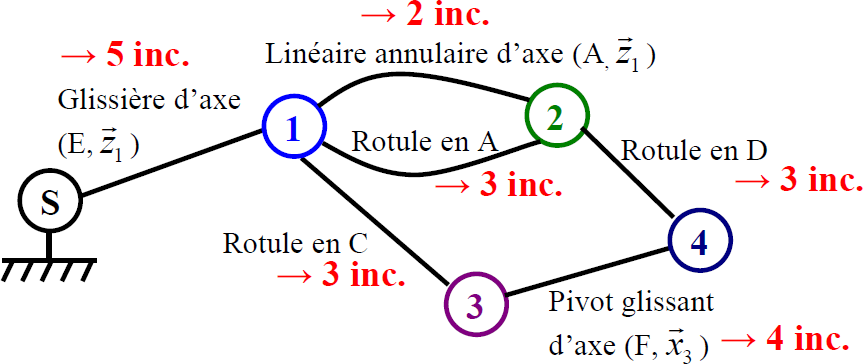
\includegraphics[width=.6\textwidth]{png/img1}
\end{center}

\paragraph{}
\textit{Donner la forme des torseurs d'actions transmissibles des liaisons 1--3, 3--4 et 2--4 dans la base 3 conformément à la notation imposée ci-dessous.}
La liaison entre 1 et 3 est une liaison rotule de centre $C$: 

$$
\left\{
F_{1 \rightarrow 3} 
\right\}=
\left\{
\begin{array}{cc}
X_{13} & 0 \\
Y_{13} & 0 \\
Z_{13} & 0 \\
\end{array}
\right\}_{C,B_3}
$$

La liaison entre 3 et 4 est une liaison pivot glissant de de centre $F$ et d'axe $\vect{x_3}$: 

$$
\left\{
F_{4 \rightarrow 3} 
\right\}=
\left\{
\begin{array}{cc}
0 & 0 \\
Y_{43} & M_{43} \\
Z_{43} & N_{43} \\
\end{array}
\right\}_{F,B_3}
$$

La liaison entre 2 et 4 est une liaison rotule de de centre $D$ : 

$$
\left\{
F_{2 \rightarrow 4} 
\right\}=
\left\{
\begin{array}{cc}
X_{24} & 0 \\
Y_{24} & 0 \\
Z_{24} & 0 \\
\end{array}
\right\}_{D,B_3}
$$
\paragraph{}
\textit{Déterminer les directions de $\vect{R_{1\rightarrow 3}}$ et de $\vect{R_{2\rightarrow 4}}$ puis en déduire des simplifications dans les torseurs précédents.}

On isole les solides $3$ et $4$. Cet ensemble est soumis à 2 forces. D'après le PFS, ces deux forces ont même norme, même direction et sens opposé. En conséquence, $X_{13}+X_{24}=0$ et $Y_{13}=Z_{13}=Y_{24}=Z_{24}=0$.

$$
\left\{
F_{1 \rightarrow 3} 
\right\}=
\left\{
\begin{array}{cc}
X_{13} & 0 \\
0 & 0 \\
0 & 0 \\
\end{array}
\right\}_{C,B_3}
\quad 
\left\{
F_{2 \rightarrow 4} 
\right\}=
\left\{
\begin{array}{cc}
X_{24} & 0 \\
0 & 0 \\
0 & 0 \\
\end{array}
\right\}_{D,B_3}
$$


\paragraph{}
\textit{Déterminer l'expression de $||\vect{R_{2\rightarrow 4}}||$ en fonction de $p$ et $S$.}
On a $||\vect{R_{2\rightarrow 4}}||=pS$ 

\paragraph{}
\textit{En isolant le solide $2$ et en utilisant le théorème du moment statique au point $A$ projetée sur $\vect{z_2}$, déterminer l'expression de $X_{42}$ en fonction de $P$ et des paramètres géométriques utiles.}
On isole le solide 2. 

On fait le bilan des actions mécaniques extérieures au point $A$ :
Liaison rotule en $A$ : 
$$
\left\{
F_{1 \rightarrow 2} 
\right\}=
\left\{
\begin{array}{cc}
X_{12} & 0 \\
Y_{12} & 0 \\
Z_{12} & 0 \\
\end{array}
\right\}_{A,B_2}
$$



Liaison linéaire annulaire au point $B$ :
$$
\left\{
F_{1 \rightarrow 2} 
\right\}=
\left\{
\begin{array}{cc}
0 & 0 \\
Y'_{12} & 0 \\
Z'_{12} & 0 \\
\end{array}
\right\}_{B,B_2}
=
\left\{
\begin{array}{cc}
0 &  -\\
Y'_{12} &  -\\
Z'_{12} &  0\\
\end{array}
\right\}_{A,B_2}
$$


Liaison rotule au point $D$ :
$$
\left\{
F_{4 \rightarrow 2} 
\right\}
=
\left\{
\begin{array}{cc}
X_{42}  & 0 \\
0 & 0 \\
0 & 0 \\
\end{array}
\right\}_{D,B_2}
=
\left\{
\begin{array}{cc}
X_{42}  & -\\
0 & -\\
0 & 0 \\
\end{array}
\right\}_{A,B_2}
$$


Pesanteur en $G$ :
$$
\left\{
F_{pes \rightarrow 2} 
\right\}
=
\left\{
\begin{array}{cc}
-P  & 0 \\
0 & 0 \\
0 & 0 \\
\end{array}
\right\}_{G,B_2}
=
\left\{
\begin{array}{cc}
-P  & -\\
0 & -  \\
0 &  \\
\end{array}
\right\}_{A,B_2}
$$

\paragraph{}
\textit{Calculer la valeur de la pression $p$ maximale pour la position $\theta=0^o$ (et donc $\gamma = 18^o$) et $\beta = 0^o$ avec les valeurs numériques données.}


\paragraph{}
\textit{Le vérin utilisé peut supporter une pression de 10 bars maximum. Conclure quant à la capacité du système à satisfaire le critère de masse de radar à déplacer.}



\section*{Griffe et lame de bulldozer}
\setcounter{paragraph}{0}


La lame 2 est rattachée au bulldozer 1 par l'intermédiaire de la pièce 3 ainsi que les deux vérins 7+6 et 5+4. La griffe 13 est rattachée au bulldozer par l'intermédiaire de la pièce 12 et du vérin 8+9. Les liaisons aux points $A$, $B$, $C$, $D$, $E$, $F$, $G$, $H$, $I$ et $J$ sont des liaisons pivots parfaites suivant l'axe $\vect{z_0}$. La pièce 12 est reliée à la griffe 13 au point $K$ grâce à une rainure. 

Tous les vérins ont une surface de piston identique de $2\, 500\pi\; mm^2$.

\paragraph{}
\textit{La terre exerce sur la griffe une action mécanique $\vect{F_{\text{sol}\rightarrow \text{griffe}}}$ au point $M$ donnée sur le document réponse. Résoudre graphiquement le problème pour déterminer la pression dans les deux vérins actionnant sur la griffe.}

\textbf{Pour les deux premières questions, vous énoncerez brièvement la démarche utilisée. De plus, vous indiquerez clairement sur le dessin les directions des efforts que vous tracez.}

\paragraph{}
\textit{La terre exerce sur la lame une action mécanique $\vect{F_{\text{sol}\rightarrow \text{lame}}}$ au point $N$ donnée sur le document réponse. Résoudre graphiquement le problème pour déterminer la pression dans les deux vérins actionnant la lame.}


\paragraph{}
\textit{Conclure vis-à-vis du cahier des charges quant aux performances obtenues.}



\section*{Echelle en appui sur un mur}

\setcounter{paragraph}{0}
\paragraph{Tous les frottements sont négligés}
\textit{Le grimpeur est situé au milieu de l'échelle. En appliquant le PFS en A à l'ensemble échelle et grimpeur, sans écrire le moindre torseur, montrer que l'échelle ne peut tenir en équilibre.}

\paragraph{On considère qu'il y a du frottement au point $A$.}
\textit{Le coefficient de frottement est égal à 0,3. Reproduire le schéma et faire apparaître le cône de frottement. Préciser la position de l'effort normal et de l'effort tangentiel à la limite du glissement.}
 

\paragraph{On considère qu'il y a du frottement au point $A$.}
\textit{Appliquer le PFS au point A à l'ensemble échelle et grimpeur, déterminer l'angle $\alpha$ pour lequel l'échelle est en équilibre.}

\paragraph{On considère qu'il y a du frottement au point $A$ et en $B$.}
\textit{Dans quelle situation se trouve le système. Pour $\alpha=20^o$, préciser pour quel poids P le système est en équilibre. Vous pourrez utiliser une méthode graphique.}

\end{document}







